\documentclass[a4paper,oneside,12pt]{report}
% Package yang diperlukan
\usepackage{graphicx}      % Untuk memasukkan gambar
\usepackage{titling}       % Untuk kustomisasi halaman judul
\usepackage{geometry}      % Untuk mengatur margin halaman
\usepackage{listings}      % Untuk menampilkan blok kode
\usepackage{xcolor}        % Untuk menggunakan warna
\usepackage{float}         % Untuk kontrol penempatan float (seperti gambar)
\usepackage{hyperref}      % Untuk membuat hyperlink (URL, referensi)
\usepackage{indentfirst}   % Untuk memberi indentasi pada paragraf pertama setiap seksi
\usepackage{url}           % Untuk format URL
\usepackage{fancyhdr}      % Untuk kustomisasi header dan footer
\usepackage{tocloft}       % Untuk kustomisasi Daftar Isi
\usepackage{bookmark}      % Untuk manajemen bookmark PDF yang lebih baik

%======================================================================
% PENGATURAN GEOMETRI HALAMAN
%======================================================================
\geometry{left=3cm, right=2.5cm, top=2cm, bottom=2.5cm}
\sloppy

%======================================================================
% PENGATURAN WARNA UNTUK BLOK KODE
%======================================================================
\definecolor{codegreen}{rgb}{0,0.6,0}
\definecolor{codegray}{rgb}{0.5,0.5,0.5}
\definecolor{codepurple}{rgb}{0.58,0,0.82}
\definecolor{backcolour}{rgb}{0.95,0.95,0.92}
\definecolor{darkblue}{rgb}{0,0,0.6}

%======================================================================
% PENGATURAN BLOK KODE (LISTINGS)
%======================================================================
\lstdefinestyle{commonstyle}{
    backgroundcolor=\color{backcolour}, 
    breakatwhitespace=false, 
    breaklines=true, 
    captionpos=b, 
    keepspaces=true,
    numbers=left, 
    numbersep=5pt, 
    showspaces=false, 
    showstringspaces=false,
    showtabs=false, 
    tabsize=2, 
    frame=single,
    basicstyle=\ttfamily\footnotesize,
    numberstyle=\tiny\color{codegray},
    columns=flexible,
    postbreak=\mbox{\textcolor{red}{$\hookrightarrow$}\space},
    breakindent=0pt,
    breakautoindent=false
}

% Gaya khusus untuk Java
\lstdefinestyle{javastyle}{
    style=commonstyle,
    language=Java,
    commentstyle=\color{codegreen},
    keywordstyle=\color{darkblue},
    stringstyle=\color{codepurple},
    emph={package,import,public,class,extends,void,private,static,return,new,throws,if,null},
    emphstyle=\color{darkblue},
    basicstyle=\ttfamily\scriptsize
}

% Gaya khusus untuk Gherkin (Cucumber Features)
\lstdefinestyle{gherkinstyle}{
    style=commonstyle,
    commentstyle=\color{codegreen},
    keywordstyle=\color{darkblue},
    stringstyle=\color{codepurple},
    emph={Feature,Scenario,Scenario Outline,Given,When,Then,And,But,Examples},
    emphstyle=\color{darkblue}\bfseries,
    basicstyle=\ttfamily\scriptsize
}

% Gaya khusus untuk XML
\lstdefinestyle{xmlstyle}{
    style=commonstyle,
    language=XML,
    commentstyle=\color{codegreen},
    keywordstyle=\color{darkblue},
    stringstyle=\color{codepurple},
    basicstyle=\ttfamily\scriptsize
}

% Gaya khusus untuk Bash
\lstdefinestyle{bashstyle}{
    style=commonstyle,
    commentstyle=\color{codegreen},
    keywordstyle=\color{darkblue},
    stringstyle=\color{codepurple},
    basicstyle=\ttfamily\scriptsize
}

%======================================================================
% PENGATURAN LAIN-LAIN
%======================================================================
% Perintah kustom untuk bingkai gambar
\newcommand{\customfbox}[1]{%
  \setlength{\fboxsep}{0pt}%
  \setlength{\fboxrule}{0.5pt}%
  \fcolorbox{black}{white}{#1}%
}

% Mengganti nama default "Figure" menjadi "Gambar"
\renewcommand{\figurename}{Gambar}
\renewcommand{\thefigure}{\arabic{figure}}

% Pengaturan Hyperlink
\hypersetup{
    colorlinks=true, 
    linkcolor=black, 
    filecolor=black, 
    urlcolor=black,
    citecolor=black,
    pdftitle={Laporan Praktikum PPPL - Cucumber dan Selenium}, 
    pdfpagemode=FullScreen, 
    breaklinks=true
}

% Pengaturan Header & Footer (nomor halaman di tengah bawah)
\pagestyle{fancy}
\fancyhf{}
\fancyfoot[C]{\thepage}
\renewcommand{\headrulewidth}{0pt}

\fancypagestyle{plain}{
    \fancyhf{}
    \fancyfoot[C]{\thepage}
    \renewcommand{\headrulewidth}{0pt}
}

%======================================================================
% PENGATURAN STRUKTUR BAB DAN DAFTAR ISI
%======================================================================
\renewcommand{\contentsname}{Daftar Isi}
\renewcommand{\bibname}{Daftar Pustaka}

% Menghilangkan nomor bab tetapi mempertahankan penomoran seksi
\renewcommand{\thechapter}{}
\renewcommand{\chaptername}{}

% Format penomoran seksi menjadi [nomor bab].[nomor seksi]
\renewcommand{\thesection}{\arabic{chapter}.\arabic{section}}
\renewcommand{\thesubsection}{\thesection.\arabic{subsection}}

\setcounter{secnumdepth}{3}
\setcounter{tocdepth}{3}

% Format Daftar Isi (TOC)
\renewcommand{\cftchapdotsep}{\cftdotsep}
\renewcommand{\cftchapleader}{\cftdotfill{\cftchapdotsep}}
\setlength{\cftchapindent}{0em}
\setlength{\cftsecindent}{2em}
\setlength{\cftsubsecindent}{4em}
\setlength{\cftchapnumwidth}{0em}
\setlength{\cftsecnumwidth}{2.5em}
\setlength{\cftsubsecnumwidth}{3.2em}
\renewcommand{\cftchappresnum}{}
\renewcommand{\cftchapaftersnum}{}

% Perintah kustom untuk membuat judul bab di TOC menjadi tebal
\newcommand{\tocboldsection}[1]{%
  \protect\renewcommand{\protect\cftchapfont}{\protect\bfseries}%
  #1%
  \protect\renewcommand{\protect\cftchapfont}{}%
}

%======================================================================
% AWAL DOKUMEN
%======================================================================
\begin{document}

% Halaman Judul
\newgeometry{left=3cm, right=2.5cm, top=2cm, bottom=2cm}
\begin{titlingpage}
    \begin{center}
        \vspace*{0.3cm}
        {\large \textbf{\MakeUppercase{Laporan Praktikum}}} \\[0.3cm]
        {\large \textbf{\MakeUppercase{Praktikum Pengujian Perangkat Lunak}}} \\[0.3cm]
        {\large \textbf{\MakeUppercase{Pertemuan 11}}} \\[0.3cm]
        {\large \textbf{\MakeUppercase{Automasi Pengujian Perangkat Lunak Menggunakan Cucumber dan Selenium}}} \\[0.8cm]

        
\includegraphics[height=7cm]{lambang ugm.png} \\[0.8cm]

        {\normalsize \textbf{Disusun oleh:}} \\[0.3cm]
        \begin{tabular}{@{}l l @{}}
            \textbf{Nama}           & : Januarsyah Akbar                                 \\
            \textbf{NIM}            & : 24/535846/SV/24314                               \\
            \textbf{Kelas}          & : B2                                               \\
            \textbf{Dosen Pengampu} & : Divi Galih Prasetyo Putri, S.Kom., M.Kom., Ph.D. \\
        \end{tabular} \\[1.5cm]

        {\normalsize \textbf{PROGRAM STUDI D-IV}} \\[0.15cm]
        {\normalsize \textbf{TEKNOLOGI REKAYASA PERANGKAT LUNAK}} \\[0.15cm]
        {\normalsize \textbf{DEPARTEMEN TEKNIK ELEKTRO DAN INFORMATIKA}} \\[0.15cm]
        {\normalsize \textbf{SEKOLAH VOKASI}} \\[0.15cm]
        {\normalsize \textbf{UNIVERSITAS GADJAH MADA}} \\[0.15cm]
        {\normalsize \textbf{YOGYAKARTA}} \\[0.15cm]
        {\normalsize \textbf{2026}}
    \end{center}
\end{titlingpage}
\restoregeometry

% Halaman kosong setelah cover (halaman i, tidak bernomor)
\clearpage
\pagenumbering{roman}
\setcounter{page}{1}
\thispagestyle{empty}

% --- Daftar Isi (halaman ii) ---
\clearpage
\setcounter{page}{2}
\addcontentsline{toc}{chapter}{Daftar Isi}
\tableofcontents
\clearpage

% Mengatur penomoran halaman menjadi arab dan mulai dari 1
\pagenumbering{arabic}
\setcounter{page}{1}

\chapter[Tujuan Praktikum]{Tujuan Praktikum}
\begin{enumerate}
    \item Memahami konsep pengujian otomatis berbasis perilaku (\textit{Behavior Driven Development}) menggunakan Cucumber.
    \item Mengonfigurasi dependensi Maven serta mengimplementasikan pola desain \textit{Page Object Model} (POM) dengan Selenium WebDriver.
    \item Merancang, mengeksekusi, dan menganalisis pengujian skenario pencarian (Latihan) serta autentikasi masuk akun (Tugas) menggunakan sintaks Gherkin bahasa Indonesia.
\end{enumerate}
\clearpage

\chapter[\texorpdfstring{\tocboldsection{Langkah Praktikum}}{Langkah Praktikum}]{Langkah Praktikum}

\section{Penambahan Dependensi di Awal Langkah}
Sebelum menulis kode pengujian, dependensi Cucumber dan Selenium dikonfigurasi di dalam file \texttt{pom.xml} proyek Maven. Penggunaan \textit{Bill of Materials} (BOM) diterapkan untuk menyelaraskan versi Cucumber secara otomatis tanpa harus mendefinisikan nomor versi pada setiap \textit{sub-dependency}.

File \texttt{pom.xml} yang dikonfigurasi berisi kode sebagai berikut:
\begin{lstlisting}[style=xmlstyle, caption={Konfigurasi Dependensi Cucumber dan Selenium di pom.xml}]
<!-- Potongan berkas pom.xml untuk Penambahan Dependensi -->
<dependencies>
    <!-- Selenium Java Driver -->
    <dependency>
        <groupId>org.seleniumhq.selenium</groupId>
        <artifactId>selenium-java</artifactId>
        <version>4.21.0</version>
    </dependency>
    <!-- Safari Driver (Opsional/Pendukung OS Mac) -->
    <dependency>
        <groupId>org.seleniumhq.selenium</groupId>
        <artifactId>selenium-safari-driver</artifactId>
        <version>4.21.0</version>
    </dependency>
    <!-- JUnit 5 API -->
    <dependency>
        <groupId>org.junit.jupiter</groupId>
        <artifactId>junit-jupiter-api</artifactId>
        <version>5.10.2</version>
        <scope>test</scope>
    </dependency>
    <!-- Cucumber Java Support -->
    <dependency>
        <groupId>io.cucumber</groupId>
        <artifactId>cucumber-java</artifactId>
        <scope>test</scope>
    </dependency>
    <!-- Cucumber JUnit Integration Runner -->
    <dependency>
        <groupId>io.cucumber</groupId>
        <artifactId>cucumber-junit</artifactId>
        <scope>test</scope>
    </dependency>
    <!-- JUnit 4 Engine untuk eksekusi Test Runner standard -->
    <dependency>
        <groupId>junit</groupId>
        <artifactId>junit</artifactId>
        <version>4.13.2</version>
        <scope>test</scope>
    </dependency>
</dependencies>
\end{lstlisting}

\section{Implementasi Page Object Model (POM)}
Untuk mendukung struktur kode yang bersih, dibuat 5 berkas kelas halaman (\textit{Page Classes}) di dalam paket \texttt{pages} pada direktori \texttt{src/main/java/pages}:

\begin{enumerate}
    \item \textbf{\texttt{basePage.java}} \\
          Merupakan kelas induk (\textit{parent class}) yang mewadahi inisialisasi \texttt{WebDriver} dan \texttt{WebDriverWait} serta mendefinisikan metode pembantu umum (\textit{generic helper methods}) agar tidak perlu dideklarasikan berulang kali di sub-kelas.
          \begin{lstlisting}[style=javastyle, caption={Implementasi Kelas basePage.java}]
package pages;

// [Import statements omitted]

public class basePage {
    WebDriver driver;
    WebDriverWait wait;

    public basePage(WebDriver driver) {
        this.driver = driver;
        this.wait = new WebDriverWait(driver, Duration.ofSeconds(5));
    }

    public WebElement waitUntil(By by) {
        wait.until(ExpectedConditions.visibilityOfElementLocated(by));
        return driver.findElement(by);
    }

    public void click(By by) {
        waitUntil(by).click();
    }

    public void sendKeys(By by, String query) {
        waitUntil(by).sendKeys(query);
    }
}
\end{lstlisting}

    \item \textbf{\texttt{searchPage.java}} \\
          Kelas representasi halaman utama mesin pencari Bing, mewarisi \texttt{basePage} dan mendefinisikan pencari lokasi (\textit{locators}) untuk kolom input pencarian dan tombol/form pencarian.
          \begin{lstlisting}[style=javastyle, caption={Implementasi Kelas searchPage.java}]
package pages;

// [Import statements omitted]

public class searchPage extends basePage {
    public searchPage(WebDriver driver) {
        super(driver);
    }

    By searchBar = By.id("sb_form_q");
    By searchForm = By.id("sb_form");

    public void enterQuery(String query) {
        sendKeys(searchBar, query);
    }

    public void submitForm() {
        waitUntil(searchForm).submit();
    }
}
\end{lstlisting}

    \item \textbf{\texttt{resultPage.java}} \\
          Kelas representasi halaman hasil pencarian Bing yang bertugas menangkap judul halaman guna proses validasi kecocokan pencarian.
          \begin{lstlisting}[style=javastyle, caption={Implementasi Kelas resultPage.java}]
package pages;

// [Import statements omitted]

public class resultPage extends basePage {
    public resultPage(WebDriver driver) {
        super(driver);
    }

    public String getPageTitle() {
        return driver.getTitle();
    }
}
\end{lstlisting}

    \item \textbf{\texttt{loginPage.java}} \\
          Kelas representasi halaman login situs SauceDemo, mendefinisikan \textit{locators} kolom pengguna, kata sandi, tombol masuk, serta kontainer pesan kesalahan (\textit{error message}).
          \begin{lstlisting}[style=javastyle, caption={Implementasi Kelas loginPage.java}]
package pages;

// [Import statements omitted]

public class loginPage extends basePage {
    public loginPage(WebDriver driver) {
        super(driver);
    }

    By usernameField = By.id("user-name");
    By passwordField = By.id("password");
    By loginButton = By.id("login-button");
    By errorMessage = By.cssSelector("[data-test='error']");

    public void enterUsername(String username) {
        sendKeys(usernameField, username);
    }

    public void enterPassword(String password) {
        sendKeys(passwordField, password);
    }

    public void clickLogin() {
        click(loginButton);
    }

    public boolean isErrorMessageDisplayed() {
        return waitUntil(errorMessage).isDisplayed();
    }
}
\end{lstlisting}
          \clearpage
    \item \textbf{\texttt{inventoryPage.java}} \\
          Kelas representasi halaman \textit{inventory} (dasbor) pasca-login di SauceDemo yang memverifikasi keberhasilan masuk lewat kemunculan daftar produk.
          \begin{lstlisting}[style=javastyle, caption={Implementasi Kelas inventoryPage.java}]
package pages;

// [Import statements omitted]

public class inventoryPage extends basePage {
    public inventoryPage(WebDriver driver) {
        super(driver);
    }

    By inventoryList = By.className("inventory_list");

    public boolean isInventoryDisplayed() {
        return waitUntil(inventoryList).isDisplayed();
    }
}
\end{lstlisting}
\end{enumerate}

\section{Pembuatan Test Runner}
Sebuah kelas bernama \texttt{RunCucumberTest.java} dibuat pada paket \texttt{runner} (\texttt{src/test/java/runner}) untuk mendefinisikan letak berkas fungsionalitas (\textit{features}), letak kelas langkah uji (\textit{glue}), serta pengaturan format keluaran (\textit{pretty} dan laporan HTML).
\begin{lstlisting}[style=javastyle, caption={Implementasi Kelas RunCucumberTest.java}]
package runner;

// [Import statements omitted]

@RunWith(Cucumber.class)
@CucumberOptions(
    features = "src/test/resources/features",
    glue = "stepDef",
    plugin = {"pretty", "html:target/cucumber-reports.html"}
)
public class RunCucumberTest {
}
\end{lstlisting}

\clearpage

\chapter[\texorpdfstring{\tocboldsection{Hasil dan Pembahasan}}{Hasil dan Pembahasan}]{Hasil dan Pembahasan}

\section{Latihan: Pengujian Fitur Pencarian (Search Feature)}
Pada sesi Latihan, skenario difokuskan pada pengujian otomatis fitur pencarian di mesin pencari Bing menggunakan sintaks Gherkin bahasa Indonesia.

\subsection{Gherkin Feature File - \texttt{search.feature}}
Berkas \texttt{search.feature} diletakkan di direktori \texttt{src/test/resources/features/search.feature}:
\begin{lstlisting}[style=gherkinstyle, caption={Skenario Uji search.feature dengan Bahasa Gherkin}]
Feature: Search functionality on Bing

  Scenario: Search for a keyword on Bing
    Given aku buka halaman pencarian Bing
    When aku ngetik kata kunci "Cucumber Java"
    And aku teken enter buat nyari
    Then harusnya muncul hasil yang ada hubungannya sama "Cucumber Java"
\end{lstlisting}

\subsection{Step Definitions - \texttt{SearchSteps.java}}
Kelas pemetaan langkah fungsional pencarian Bing diimplementasikan di \texttt{src/test/java/stepDef/SearchSteps.java}:
\begin{lstlisting}[style=javastyle, caption={Implementasi Kelas Langkah Uji SearchSteps.java}]
package stepDef;

// [Import statements omitted]

public class SearchSteps {
    WebDriver driver;
    searchPage search;
    resultPage result;

    @Given("aku buka halaman pencarian Bing")
    public void iAmOnTheBingSearchPage() {
        driver = new ChromeDriver();
        driver.manage().timeouts().implicitlyWait(Duration.ofSeconds(10));
        driver.get("https://www.bing.com");
        search = new searchPage(driver);
    }

    @When("aku ngetik kata kunci {string}")
    public void iEnterTheSearchQuery(String query) {
        search.enterQuery(query);
    }

    @And("aku teken enter buat nyari")
    public void iSubmitTheSearchForm() {
        search.submitForm();
    }

    @Then("harusnya muncul hasil yang ada hubungannya sama {string}")
    public void iShouldSeeResultsRelatedTo(String query) {
        result = new resultPage(driver);
        String title = result.getPageTitle();
        Assert.assertTrue("Judul halaman '" + title + "' gak ada hubungannya sama '" + query + "'", 
            title.toLowerCase().contains(query.toLowerCase()));
        driver.quit();
    }
}
\end{lstlisting}

\subsection{Hasil Pengujian Fitur Pencarian}
Eksekusi pengujian dilakukan melalui kelas \texttt{RunCucumberTest}. Hasil pengujian fungsionalitas pencarian Bing berjalan sukses dengan indikasi centang hijau dan semua asersi lulus uji (\textit{PASSED}).

\begin{figure}[H]
    \centering
    \customfbox{
\includegraphics[width=0.85\textwidth]{screenshot step/Latihan_test_result.png}}
    \caption{Hasil Eksekusi Pengujian Fitur Pencarian Bing}
    \label{fig:latihan_result}
\end{figure}

\clearpage

\section{Tugas: Pengujian Fitur Login (Login Feature)}
Pada bagian Tugas Mandiri, skenario difokuskan untuk menguji fitur autentikasi pada platform e-commerce sandbox SauceDemo. Pengujian dirancang mencakup dua kondisi: skenario masuk sukses (positif) menggunakan \textit{Scenario Outline} dengan contoh data, dan skenario masuk gagal (negatif).

\subsection{Gherkin Feature File - \texttt{login.feature}}
Berkas \texttt{login.feature} diletakkan di direktori \texttt{src/test/resources/features/login.feature}:
\begin{lstlisting}[style=gherkinstyle, caption={Skenario Uji login.feature dengan Scenario Outline}]
Feature: Login functionality for SauceDemo

  Scenario Outline: Successful login with valid credentials
    Given aku lagi di halaman login SauceDemo
    When aku masukin username "<username>" sama password "<password>"
    And aku klik tombol loginnya
    Then aku harusnya langsung masuk ke halaman inventory

    Examples:
      | username      | password     |
      | standard_user | secret_sauce |

  Scenario: Login failure with invalid credentials
    Given aku lagi di halaman login SauceDemo
    When aku masukin username "user_ngasal" sama password "pass_ngasal"
    And aku klik tombol loginnya
    Then harusnya muncul pesan error
\end{lstlisting}
\clearpage
\subsection{Step Definitions - \texttt{LoginSteps.java}}
Kelas implementasi langkah fungsional untuk autentikasi login SauceDemo ditulis pada \texttt{src/test/java/stepDef/LoginSteps.java}:
\begin{lstlisting}[style=javastyle, caption={Implementasi Kelas Langkah Uji LoginSteps.java}]
package stepDef;

// [Import statements omitted]

public class LoginSteps {
    WebDriver driver;
    loginPage login;
    inventoryPage inventory;

    @Given("aku lagi di halaman login SauceDemo")
    public void iAmOnTheSauceDemoLoginPage() {
        driver = new ChromeDriver();
        driver.manage().timeouts().implicitlyWait(Duration.ofSeconds(10));
        driver.get("https://www.saucedemo.com/");
        login = new loginPage(driver);
    }

    @When("aku masukin username {string} sama password {string}")
    public void iEnterUsernameAndPassword(String username, String password) {
        login.enterUsername(username);
        login.enterPassword(password);
    }

    @And("aku klik tombol loginnya")
    public void iClickTheLoginButton() {
        login.clickLogin();
    }

    @Then("aku harusnya langsung masuk ke halaman inventory")
    public void iShouldBeRedirectedToTheInventoryPage() {
        inventory = new inventoryPage(driver);
        Assert.assertTrue("Halaman inventory gak muncul nih", inventory.isInventoryDisplayed());
        driver.quit();
    }

    @Then("harusnya muncul pesan error")
    public void iShouldSeeAnErrorMessage() {
        Assert.assertTrue("Pesan error malah gak ada", login.isErrorMessageDisplayed());
        driver.quit();
    }
}
\end{lstlisting}
\clearpage
\subsection{Hasil Pengujian Fitur Login}
Pengujian dijalankan secara otomatis dengan JUnit Runner. Hasil eksekusi menunjukkan kedua skenario autentikasi berhasil diselesaikan tanpa kesalahan (\textit{All Passed}):

\begin{figure}[H]
    \centering
    \customfbox{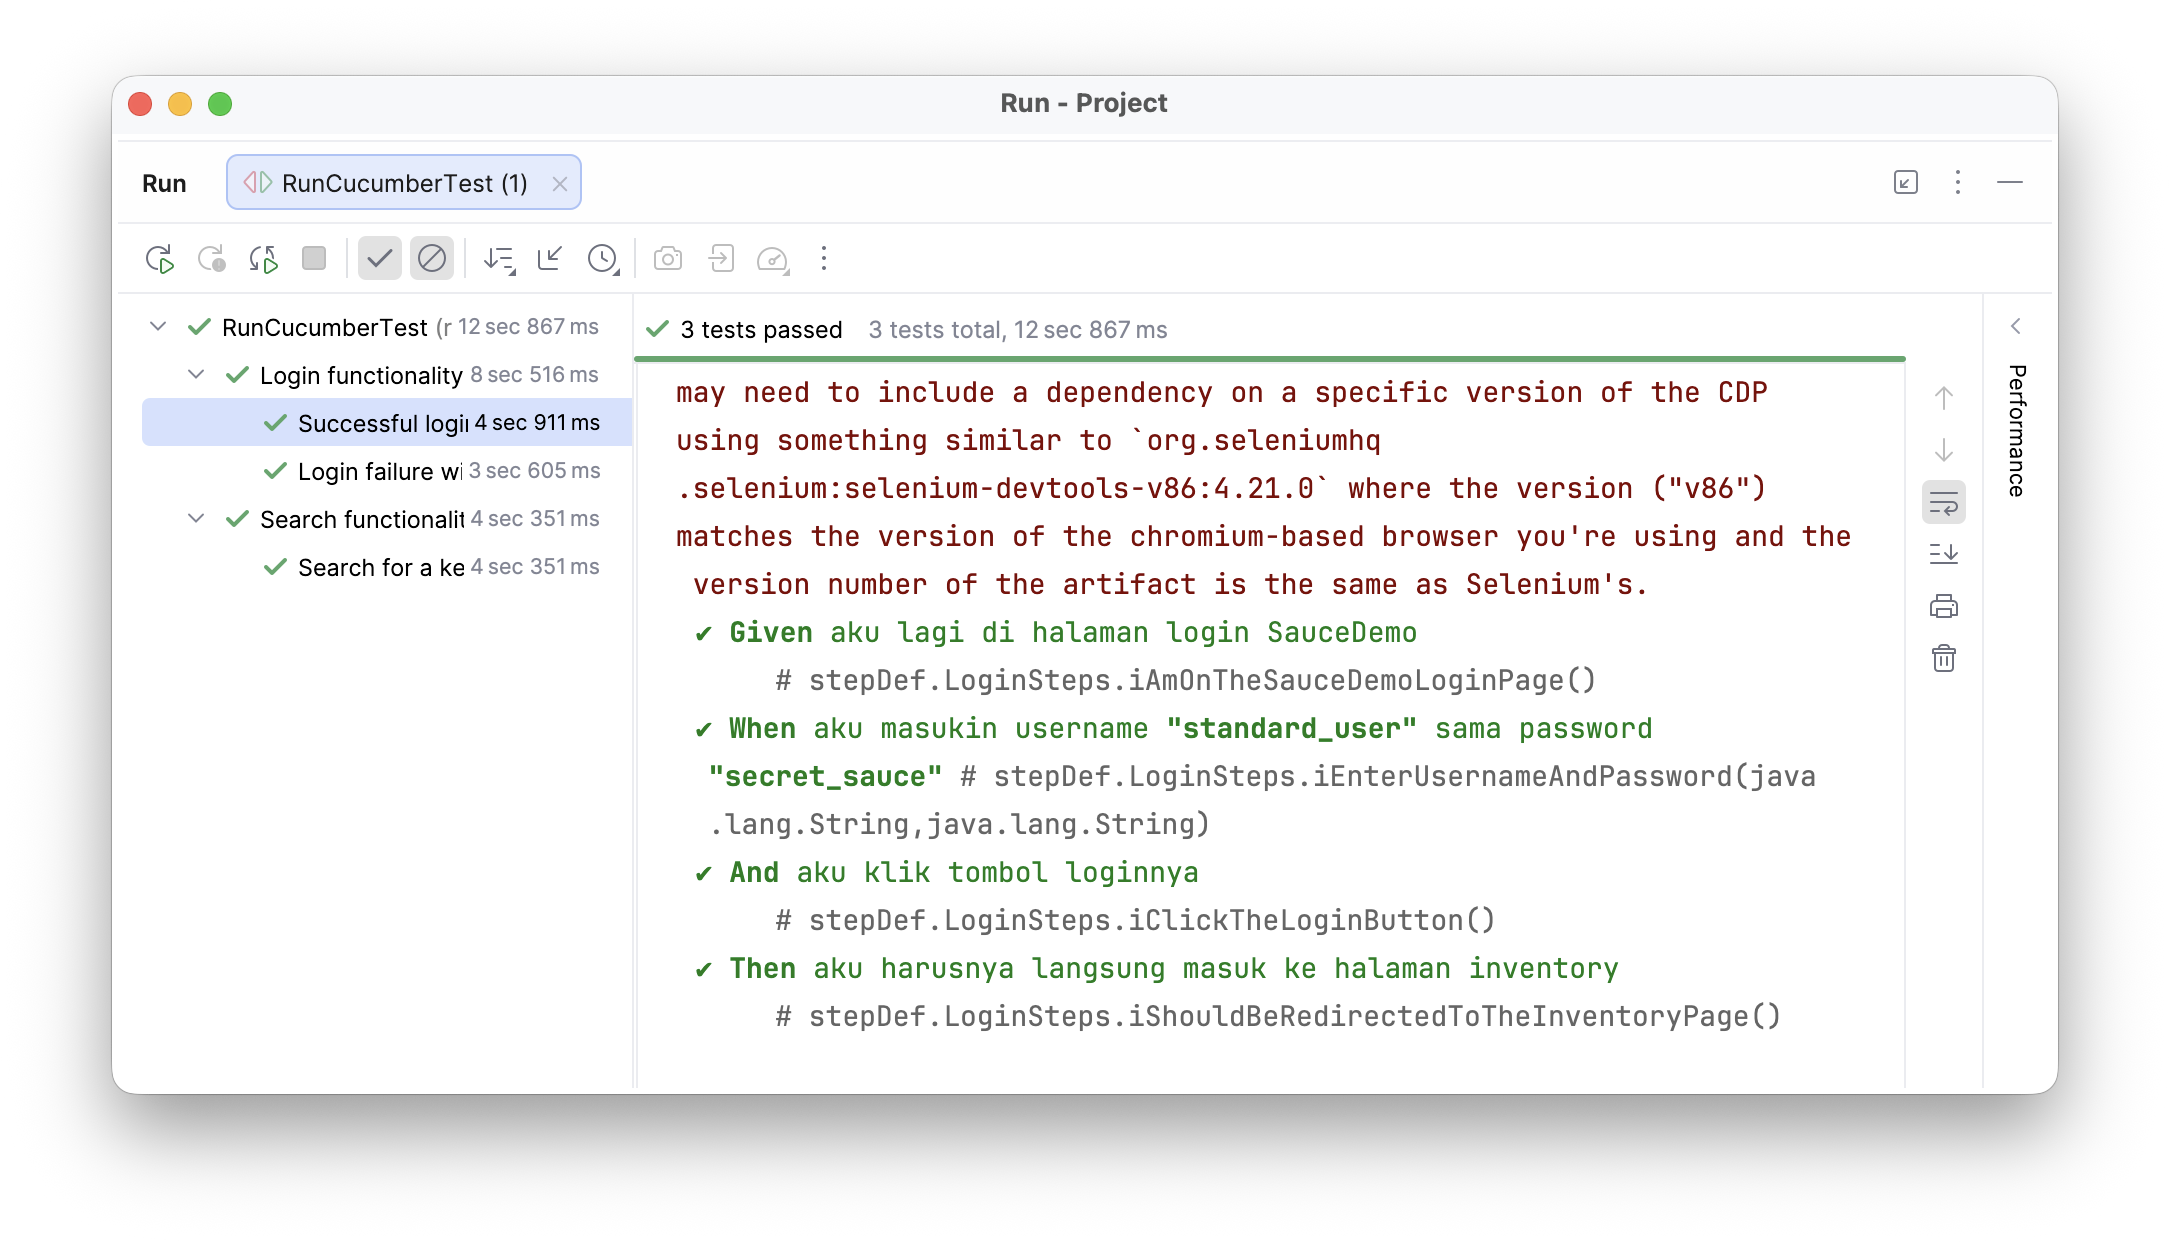
\includegraphics[width=0.85\textwidth]{screenshot step/Tugas_test_result_success.png}}
    \caption{Hasil Eksekusi Skenario Login Berhasil (Positive Case)}
    \label{fig:tugas_result_success}
\end{figure}

\begin{figure}[H]
    \centering
    \customfbox{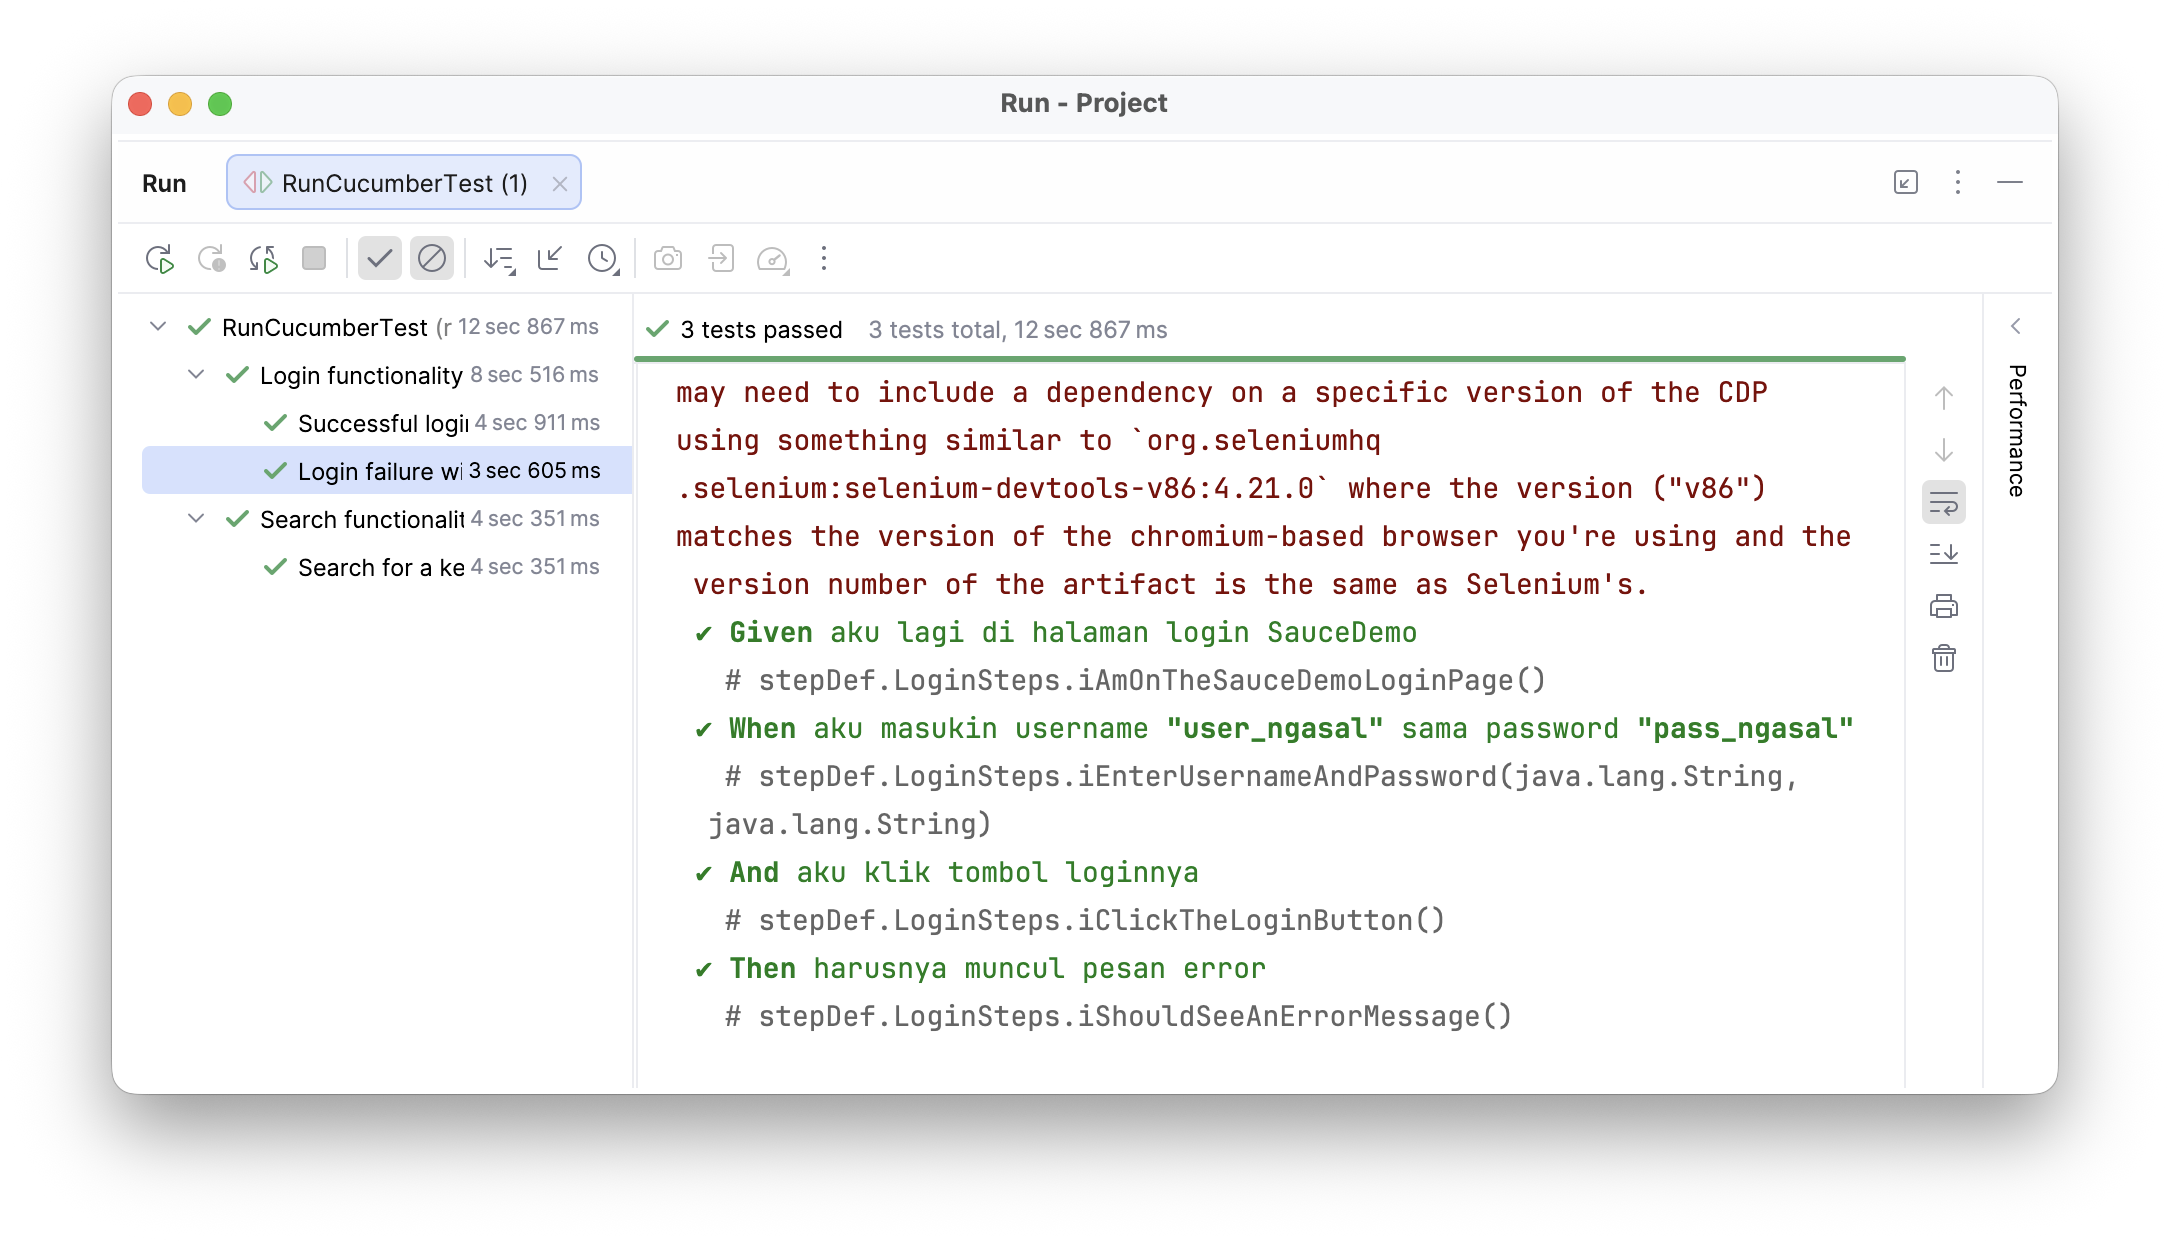
\includegraphics[width=0.85\textwidth]{screenshot step/Tugas_test_result_failure.png}}
    \caption{Hasil Eksekusi Skenario Login Gagal (Negative Case)}
    \label{fig:tugas_result_failure}
\end{figure}

\clearpage

\chapter{Kesimpulan}
Praktikum Pertemuan 11 ini berhasil mempraktikkan proses automasi pengujian menggunakan \textbf{Cucumber} dan \textbf{Selenium WebDriver} dengan pendekatan \textbf{Behavior Driven Development} (BDD) dan pola desain \textbf{Page Object Model} (POM).

Proyek berhasil dikonfigurasi menggunakan Maven dengan mendefinisikan versi Cucumber \texttt{7.34.3} dan Selenium \texttt{4.21.0} secara selaras. Implementasi skenario pencarian Bing (Latihan) dan skenario masuk akun SauceDemo (Tugas) yang didefinisikan dalam sintaks Gherkin bahasa Indonesia telah terbukti berjalan dengan sukses, asersi lulus 100\%, dan tercatat dalam berkas laporan pengujian otomatis secara komprehensif. Penerapan pola POM terbukti mempermudah perawatan kode uji dengan memisahkan representasi elemen laman dari alur logika skenario pengujian fungsional.



\end{document}
